The findings of this work allowed the authors to formulate the following conclusions:
\begin{itemize}
  \item[\textbullet]Among all tested applications IPF is the least I/O demanding. For the reference architecture it shows scalability up to 700 cores. On the other hand, other selected processors scale in the range of the number of physical cores so we expect that using them in a multinode configuration will result in similar behaviour as for the reference testbed.
  \item[\textbullet]Green Growth-pilot applications are dominated by I/O operations (mostly output) where a large HDF5 file is created and to which all processes save data;
  \item[\textbullet]Results obtained for ABMS4py - another social simulation application prove it should be subject to major improvements. For instance, the best execution time on Intel\textregistered\ Xeon\textregistered\ Gold 6140 is observed for only 9 MPI processes, whereas the testbed includes 72 physical cores (2-node configuration with 2 chips each, 18 cores per one chip)
  \item[\textbullet]OpenSWPC benchmark for given input configuration reports good scalability. It is especially illuminative in case of the reference testbed where the execution time decreases along number of cores used until maximum number of 1400 is used. Other processors show similar behaviour. Using hyper threads (where possible) does not provide any further time improvements.
  \item[\textbullet]CCTM is I/O dominated (especially output) application and, thus, the impact on the execution times is high
  \item[\textbullet]CM1 results indicate a relationship between the problem size (weather map grid) and the processors mesh, as well as the dependence between the number of threads and nesting of cores in different levels of cache. 
  \item[\textbullet]HWRF demonstrates very similar results to CM1 in terms of scalability on processors equipped with the implementation of simultaneous multithreading 
  \item[\textbullet]Best execution times are usually achieved (when considering single nodes) for the number of processes equal to the number of cores: 64 for 2-node ARM Hi1616 and 1-node AMD Epyc\textsuperscript{TM}, 72 for 2-node Intel\textregistered\ Xeon\textregistered\ Gold 6140, 20 for 2-processor 1-node Power8+;
  \item[\textbullet]In most cases hyper threading does not bring any performance improvements.
\end{itemize}
\  \\
For the final comparative analysis two additional metrics have been introduced: 
\begin{itemize}
  \item[\textbullet]\textit{Energy efficiency} calculated as a product of walltimes and TDP products which scales and binds the achieved timing results by processors by the theoretical heat generated during the tests and/or the energy consumed by processors.
  \item[\textbullet]\textit{Cost efficiency} using scaled timing results by the cores price falling on the given number of cores (cores price is calculated by dividing processor price by a given number of processor cores).
\end{itemize}

\begin{figure*}[!ht]
\centering
%% 1 line
\begin{subfigure}[t]{0.48\textwidth}
\centering
%%  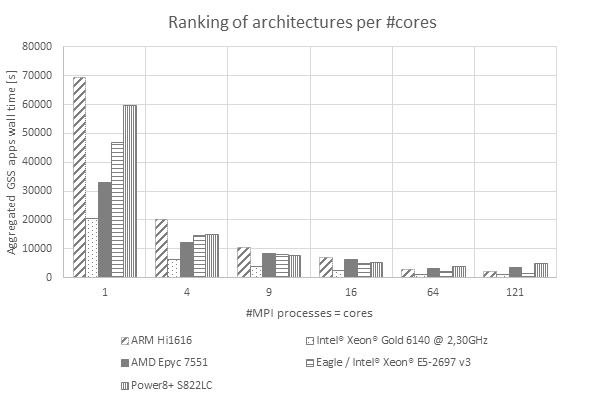
\includegraphics[width=1.\textwidth]{rank_archs_per_cores}
    \begin{tikzpicture}
    \begin{axis}[
    	xtick={1,2,3,4,5,6},
    	xticklabels={1,4,9,16,64,121},
    	xlabel=\#MPI processes \= cores,
    	ylabel=Aggregated GSS apps wall time {[s]},
     	enlarge x limits=0.15,
     	ymin=0,
    	legend style={at={(0.5,-0.2)},
    	    anchor=north,legend columns=2},
      ybar=0pt,
      bar width=0.15cm, width=1.0\textwidth
    ]
    %Arm
    \addplot[black, pattern=horizontal lines]
    coordinates {(1,69475)(2,20195)(3,10571)(4,6877)(5,2750)(6,2165)};
    %Intel gold
    \addplot[black, pattern=north west lines]
    coordinates {(1,20624)(2,6428)(3,3616)(4,2526)(5,1140)(6,1249)};
    %AMD
    \addplot[black, pattern=bricks]
    coordinates {(1,33046)(2,12036)(3,8210)(4,6234)(5,3186)(6,3546)};
    %Eagle
    \addplot[black, pattern=dots]
    coordinates {(1,46790)(2,14646)(3,7874)(4,5393)(5,1934)(6,1487)};
    %Power8
    \addplot[black, pattern=north east lines]
    coordinates {(1,59679)(2,14838)(3,7669)(4,5318)(5,4015)(6,4995)};
    \legend{Arm Hi1616, Intel Xeon Gold 6140, AMD Epyc 7551, Eagle/Intel Xeon E5-2697 v3, Power8+ S822LC}
    \end{axis}
    \end{tikzpicture}
  \caption{Ranking of architectures across number of cores (processes)}\label{fig:rankarchspercore}
\end{subfigure}\hfill
\begin{subfigure}[t]{0.48\textwidth}
%%  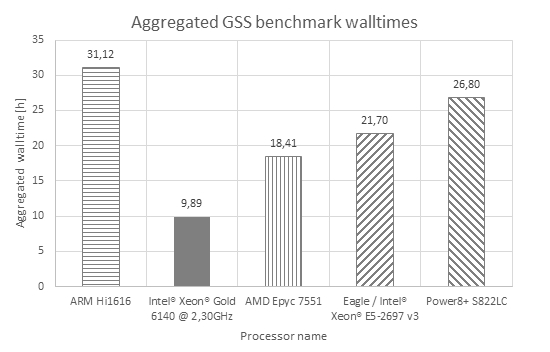
\includegraphics[width=1.\textwidth]{rank_archs_walltimes}
    \begin{tikzpicture}
    \begin{groupplot}[
    legend columns=2,
    legend entries={Arm Hi1616, Intel Xeon Gold 6140, AMD Epyc 7551, Eagle/Intel Xeon E5-2697 v3, Power8+ S822LC},
    legend style={at={(0.5,-0.2)},
    	    anchor=north,legend columns=2},
    area legend,
    group style={
    xlabels at=edge bottom,
    ylabels at=edge left,
    xticklabels at=edge bottom},
    xtick = {1,2,3,4,5},
    ymajorgrids=true,
    nodes near coords,
    every node near coord/.append style={font=\tiny},
    xlabel={Processor name},
    ylabel={Aggregated wall times {[h]}},
    ]
    \nextgroupplot[bar width=20pt, xticklabel=\empty]
    \addplot[ybar, pattern=horizontal lines] coordinates {  (1, 31.12)};
    \addplot[ybar, pattern=north west lines] coordinates { (2, 9.88)};
    \addplot[ybar, pattern=bricks] coordinates {(3, 18.41)};
    \addplot[ybar, pattern=dots] coordinates {(4, 21.70)};
    \addplot[ybar, pattern=north east lines] coordinates {  (5, 26.8)};
    \end{groupplot}
    \end{tikzpicture}
  \caption{Aggregated GSS benchmark walltimes}
  \label{fig:rankarchswalltimes}
  \end{subfigure}
\begin{subfigure}[t]{0.48\textwidth}
%  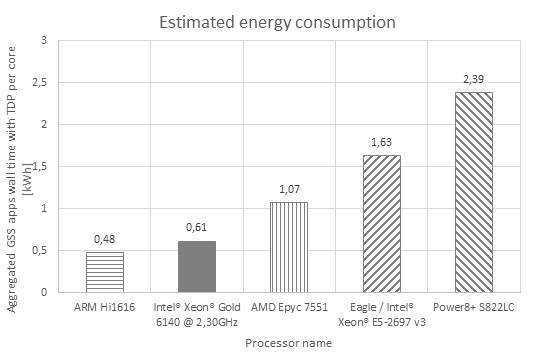
\includegraphics[width=1.\textwidth]{estimated_energy_consumption}
    \begin{tikzpicture}
    \begin{groupplot}[
        legend columns=2,
        legend entries={Arm Hi1616, Intel Xeon Gold 6140, AMD Epyc 7551, Eagle/Intel Xeon E5-2697 v3, Power8+ S822LC},
        legend style={at={(0.5,-0.2)},
        	    anchor=north,legend columns=2},
        area legend,
        group style={
            xlabels at=edge bottom,
            ylabels at=edge left,
            xticklabels at=edge bottom},
        xtick = {1,2,3,4,5},
        ymajorgrids=true,
        nodes near coords,
        every node near coord/.append style={font=\tiny},
        xlabel={Processor name},
        ylabel={Aggregated GSS apps wall time per TDP per core {[kWh]}},
    ]
    \nextgroupplot[bar width=20pt, xticklabel=\empty]
    \addplot[ybar, pattern=horizontal lines] coordinates {  (1, 0.48)};
    \addplot[ybar, pattern=north west lines] coordinates { (2, 0.61)};
    \addplot[ybar, pattern=bricks] coordinates {(3, 1.07)};
    \addplot[ybar, pattern=dots] coordinates {(4, 1.63)};
    \addplot[ybar, pattern=north east lines] coordinates {  (5, 2.39)};
    \end{groupplot}
    \end{tikzpicture}
  \caption{Ranking of architectures based on estimated energy consumption (total power needed by CPU to finish all tests) - lower is better}
  \label{fig:estimatedenergyconsumption}
  \end{subfigure}\hfill
  %% 2 line
  \begin{subfigure}[t]{0.48\textwidth}
  \centering
%  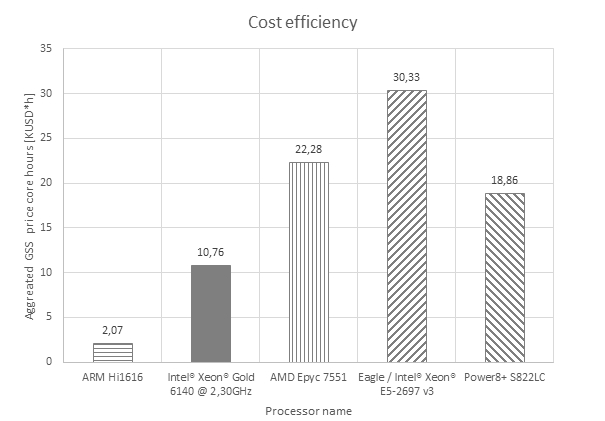
\includegraphics[width=1.\linewidth]{cost_efficiency}
    \begin{tikzpicture}
    \begin{groupplot}[
        legend columns=2,
        legend entries={Arm Hi1616, Intel Xeon Gold 6140, AMD Epyc 7551, Eagle/Intel Xeon E5-2697 v3, Power8+ S822LC},
        legend style={at={(0.5,-0.2)},
        	    anchor=north,legend columns=2},
        area legend,
        group style={
            xlabels at=edge bottom,
            ylabels at=edge left,
            xticklabels at=edge bottom},
        xtick = {1,2,3,4,5},
        ymin=0,
        ymajorgrids=true,
        nodes near coords,
        every node near coord/.append style={font=\tiny},
        xlabel={Processor name},
        ylabel={Aggreated GSS  price core-hours {[KUSD*h]}},
    ]
    \nextgroupplot[bar width=20pt, xticklabel=\empty]
    \addplot[ybar, pattern=horizontal lines] coordinates {  (1, 2.07)};
    \addplot[ybar, pattern=north west lines] coordinates { (2, 10.67)};
    \addplot[ybar, pattern=bricks] coordinates {(3, 22.28)};
    \addplot[ybar, pattern=dots] coordinates {(4, 30.33)};
    \addplot[ybar, pattern=north east lines] coordinates {  (5, 18.86)};
    \end{groupplot}
    \end{tikzpicture}    
  \caption{Ranking of architectures based on cost efficiency}
  \label{fig:costefficiency}
 \end{subfigure}%
 \bigbreak
 \caption{Benchmarking summary results}
\end{figure*}

In the scope of \textit{aggregated execution times} for the given number of cores it can be noted that in the whole range of the number of cores the winner is Intel\textregistered\ Xeon\textregistered\ Gold 6140 (Figure~\subref{fig:rankarchspercore}). Surprisingly, the AMD Epyc\textsuperscript{TM} is slower than the ARM Hi1616 when 64 or more cores are used and is also slower than the reference Intel\textregistered Xeon\textregistered\ E5-2697 when 9 or more cores are used.



By looking at the aggregated execution times across all tested applications, the winner turned out to be Intel\textregistered\ Xeon\textregistered\ Gold 6140 (Figure~\subref{fig:rankarchswalltimes}).



For the \textit{estimated cumulative energy consumption} (calculated as a sum of walltimes and TDP per used cores products expressed in kilowatt-hours) metric the winning processor is ARM Hi1616 representing the current tendency in HPC, where attention is turned to - generally speaking - energy efficient technologies. The second place winner is Intel\textregistered Xeon\textregistered\ Gold 6140 and Power8+ brings up the rear (Figure~\subref{fig:estimatedenergyconsumption}). 

The estimated power consumption chart is a good point of view when talking about green HPC computing. The presented results not exact, because they are dictated only by the estimated values based on the CPU's TDP. Nevertheless, assuming that almost all architectures use the same memory model - DDR4, it can be considered that most of the energy consumed is the energy utilized by the processor. In this scope, the best energy consumption ratio is characterized by the ARM architecture, which is absolutely designed for energy-saving solutions that is also widely used in mobile devices. The results for the new Intel Skylake architecture were a big surprise, which took the second place with a very similar result of about 20\% more. The AMD Epyc\textsuperscript{TM} presented a much worse result, but from our observations its internal architecture is better suited to applications in which I/O systems play an important role.

Another valuable finding is based on GSS cost efficiency analysis (Figure~\subref{fig:costefficiency}). ARM Hi1616 turned out to be approximately 9 times better than for Power8+ (with DDR3 and not utilized NVLinks) and 15 times better than the reference Intel\textregistered\ Xeon\textregistered\ E5-2697 processor, mostly due to its small number of expensive cores and relatively middling timing results.
Additionally, when talking about general processor characteristics extracted from all the tests performed, IBM Power8+ demonstrates particularly good performance for the applications with a big number of I/O such as Pandora, OpenSWPC, CMAQ/CCTM. The best results are obtained when the total output dominates over the input and RAM consumption. In many cases, it outperforms ARM Hi1616, Intel\textregistered\ Xeon\textregistered\ E5-2697, and AMD Epyc\textsuperscript{TM} for I/O intensive applications. On the other hand, Power8+ shows worse results than the above-mentioned processors if the applications are computationally extensive while producing a relatively small amount of output. This is the case of the IPF and ABMS applications. On all processors, all benchmarks show the highest efficiency if the number of MPI processes is between 2 and the total number of physical cores. After that, the efficiency usually drops remarkably as hyper threading is not utilised properly. At the same time, quite often the highest speedup is reached when the number of MPI processes is significantly more than 20. It would be interesting to perform the tests on the testbeds including more nodes. 



When analysed simultaneously, all the above results prove that the most promising ARM processor in the context of cost and energy consumption is the slowest at the same time (mostly due to low clock frequency). Other competitor, Intel\textregistered\ Xeon\textregistered\ Gold 6140, is 5 times less cost efficient for GSS benchmark and slightly worse in the energy consumption but it is approximately 3 times quicker regarding the aggregated execution time. In other words, the future HPC investors having the above information in place have the ability to decide which direction to follow: reach high compute intensity, minimize costs, or try to find the golden mean.

Table~\ref{tab:ranking} presents the summarised results for each individual architecture in three separate domains: walltime, energy efficiency and cost efficiency. The numbers reflects the weighted points referring to the overall applications results in a given category (in this case the less is better). In general, the most promising processor is Intel\textregistered\ Xeon\textregistered\ Gold 6140 but those individuals for whom costs and environmental aspects are the most important should look closely at ARM Hi1616.
    
    
\begin{table}
\caption{Ranking of all tested architectures (\textit{less is better})}
\label{tab:ranking}
\centering
\begin{tabular}{l|c|c|c|}
\cline{2-4}
 & \textbf{Walltime} & \textbf{\begin{tabular}[c]{@{}c@{}}Energy\\ efficiency\end{tabular}} & \textbf{\begin{tabular}[c]{@{}c@{}}Cost\\ efficiency\end{tabular}} \\ \hline
\multicolumn{1}{|l|}{\textbf{ARM Hi1616}} & 1.0 & 0.2 & 0.1 \\ \hline
\multicolumn{1}{|l|}{\textbf{Intel\textregistered\ Xeon\textregistered\ Gold 6140}} & 0.3 & 0.3 & 0.4 \\ \hline
\multicolumn{1}{|l|}{\textbf{AMD Epyc\textsuperscript{TM} 7551}} & 0.6 & 0.4 & 0.7 \\ \hline
\multicolumn{1}{|l|}{\textbf{Intel\textregistered\ Xeon\textregistered\ E5-2697}} & 0.7 & 0.7 & 1.0 \\ \hline
\multicolumn{1}{|l|}{\textbf{Power8+ S822LC}} & 0.9 & 1.0 & 0.6 \\ \hline
\end{tabular}
\end{table}

 In general, it can be said, the most promising processor is Intel\textregistered\ Xeon\textregistered\ Gold 6140 but those individuals for whom costs and environmental aspects are the most important should look closely at ARM Hi1616.

